Une visionneuse, comme Mirador, s’implémente par un module propre à Omeka. Plus qu’un module, il convient plus précisément d’en télécharger trois pour que la visionneuse soit en capacité d’afficher convenablement un manifeste IIIF~:
\begin{itemize}
	\item \texttt{le module Common\footnote{https://gitlab.com/Daniel-KM/Omeka-S-module-Common}}~: qui permet de gérer les fonctionnalités internes utilisées dans divers modules (fonctions en bloc, éléments de formulaire, assistants de vue, tâches uniques pour l'installation et les paramètres, etc.), de sorte qu'il évite au développeur de copier-coller du code commun entre les modules.\par
	\item \texttt{le module IIIF Server\footnote{https://gitlab.com/Daniel-KM/Omeka-S-module-IiifServer}}~: qui intègre les spécifications IIIF pour permettre de traiter et de partager instantanément des images de toute taille et de tout support (pdf, audio, vidéo, 3D...) dans les formats souhaités.\par
	\item \texttt{le module Mirador\footnote{https://gitlab.com/Daniel-KM/Omeka-S-module-Mirador}~:} une visionneuse en ligne avancée, qui affiche des images, des livres, des cartes, etc. via la norme IIIF. La visionneuse est multi-fenêtres, avec la possibilité de zoomer, d'afficher, de comparer et d'annoter des images.
\end{itemize}\par

Les deux derniers modules doivent être paramétrés pour qu’ils puissent lire un manifeste tiers. Il faut, pour ce faire, définir pour propriété du \enquote{Dublin Core~: A un format}.\par
\begin{figure}[H]
	\centering
	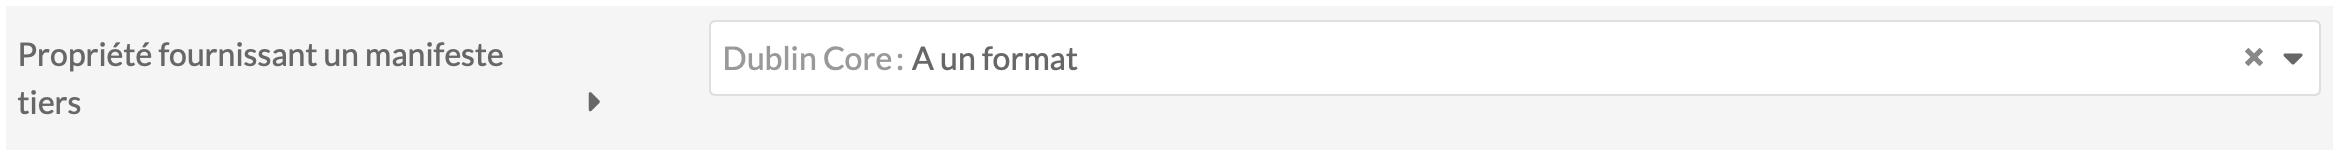
\includegraphics[width=\textwidth]{./textes/annexe/omeka-format.jpg}
	\label{fig:info}
\end{figure}

Pour ajouter un manifeste à une collection sur Omeka, il faut se rendre dans l’onglet \enquote{ressources}, \enquote{contenus}, puis \enquote{ajouter un contenu}.\par Ensuite, tout se fait dans l’onglet \enquote{valeurs}. Après avoir attribué un titre à l’objet, il convient de rechercher la propriété \enquote{a un format} de Dublin Core pour ajouter le manifeste.\par

\begin{figure}[H]
	\centering
	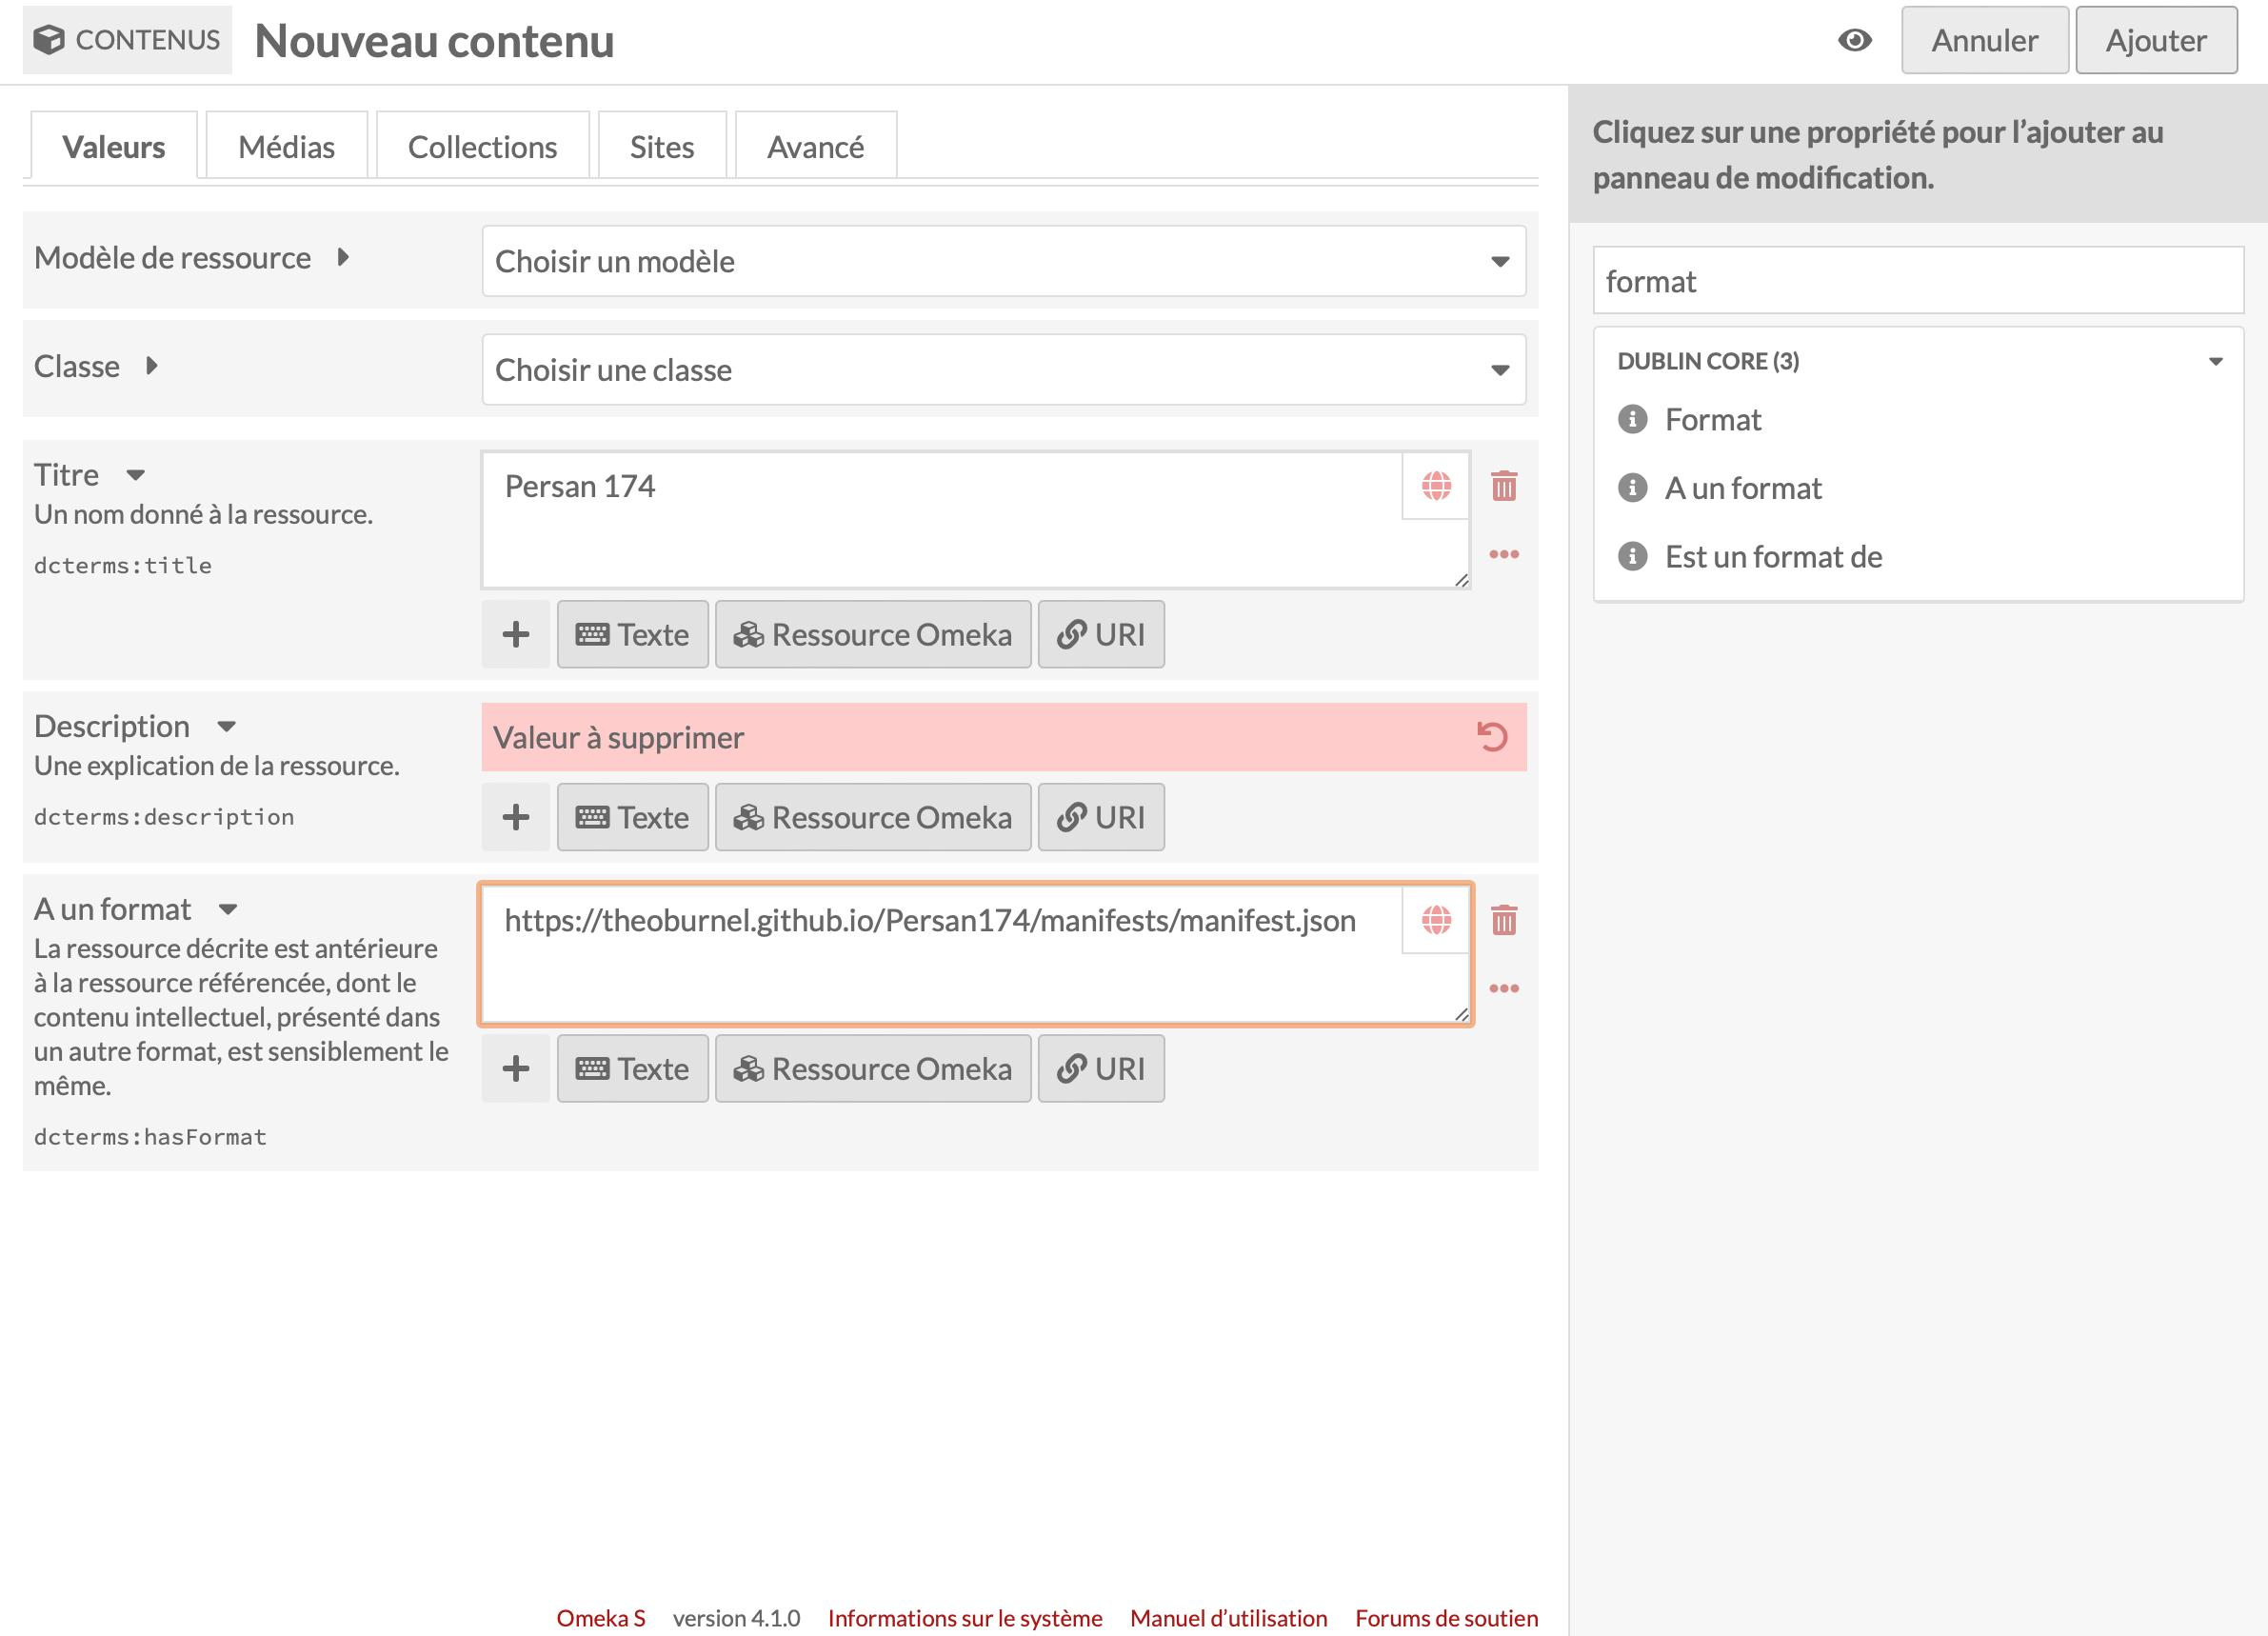
\includegraphics[scale=0.15]{./textes/annexe/omeka-item.jpg}
	\label{fig:info}
\end{figure}

Pour faire apparaître le manifeste IIIF sur la page internet, il suffit d’ajouter un bloc \enquote{Mirador Viewer} et de mettre comme pièce jointe le manifeste souhaité. Après l’enregistrement, le manifeste et les annotations apparaissent.\par

\begin{figure}[H]
	\centering
	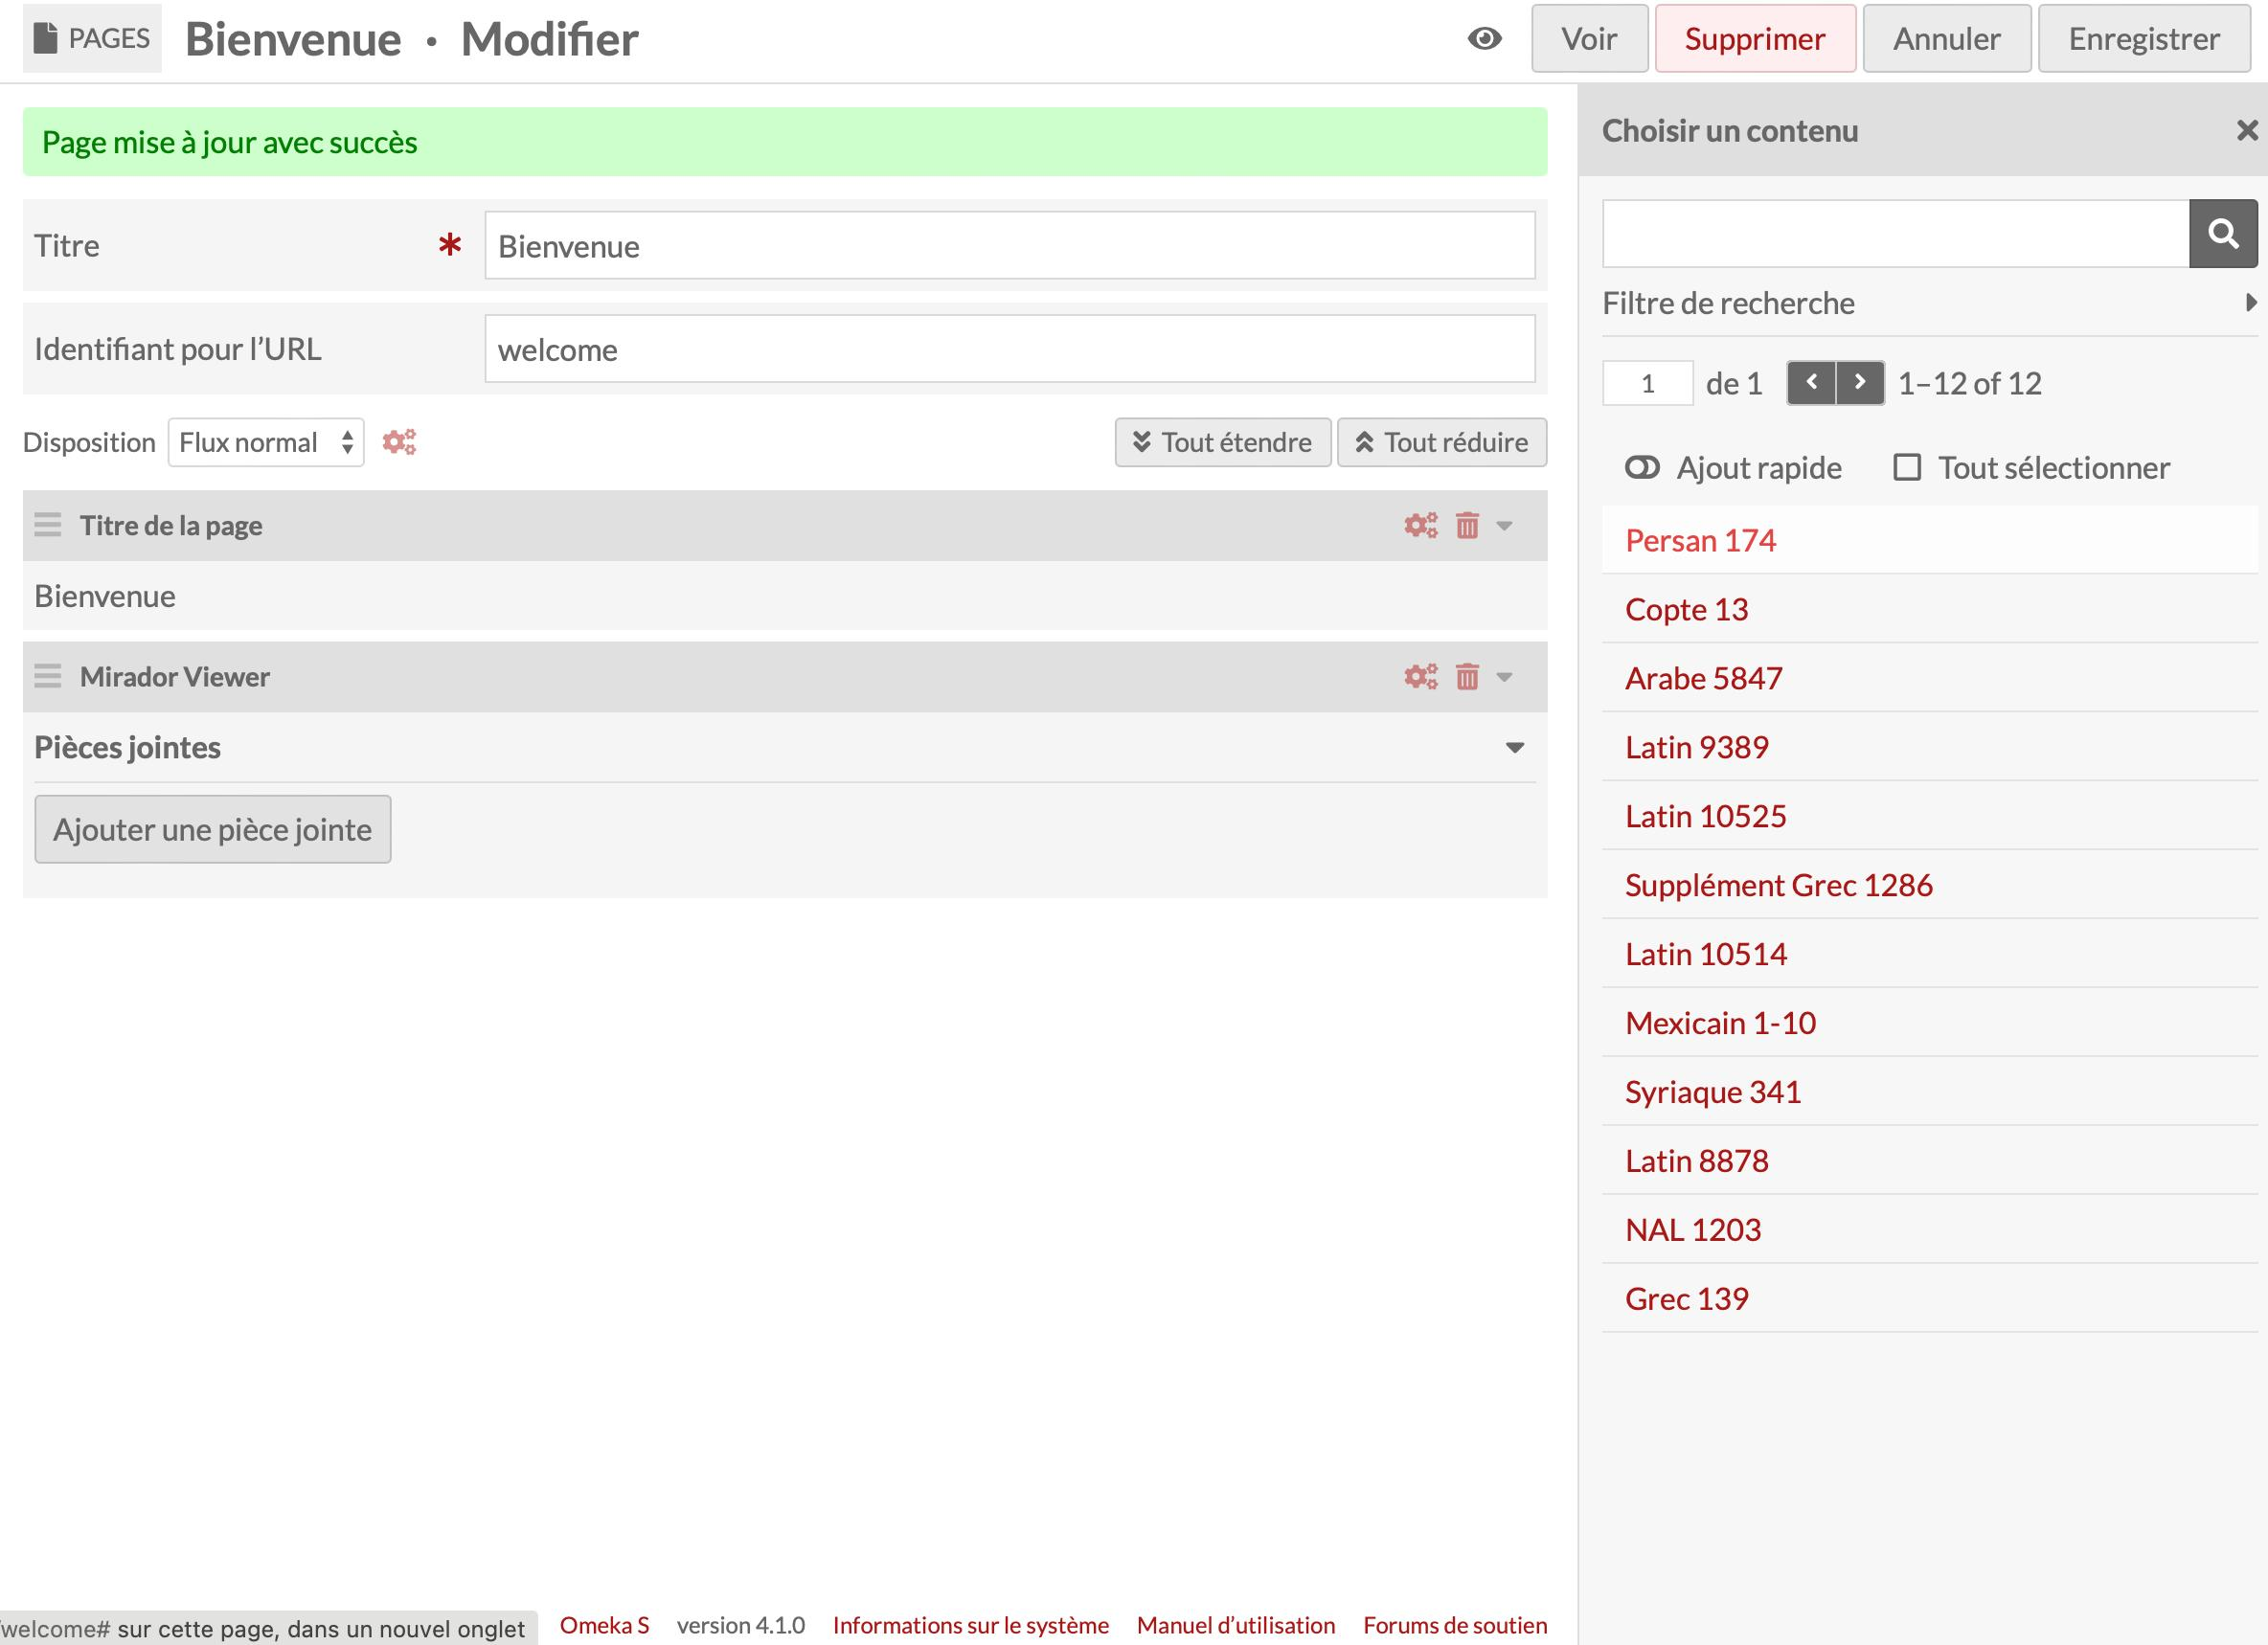
\includegraphics[scale=0.15]{./textes/annexe/omeka-visu.jpg}
	\label{fig:info}
\end{figure}

Ci-dessous, un exemple d’une visualisation d’une image IIIF sur Omeka S avec la visionneuse Mirador.

\begin{figure}[H]
	\centering
	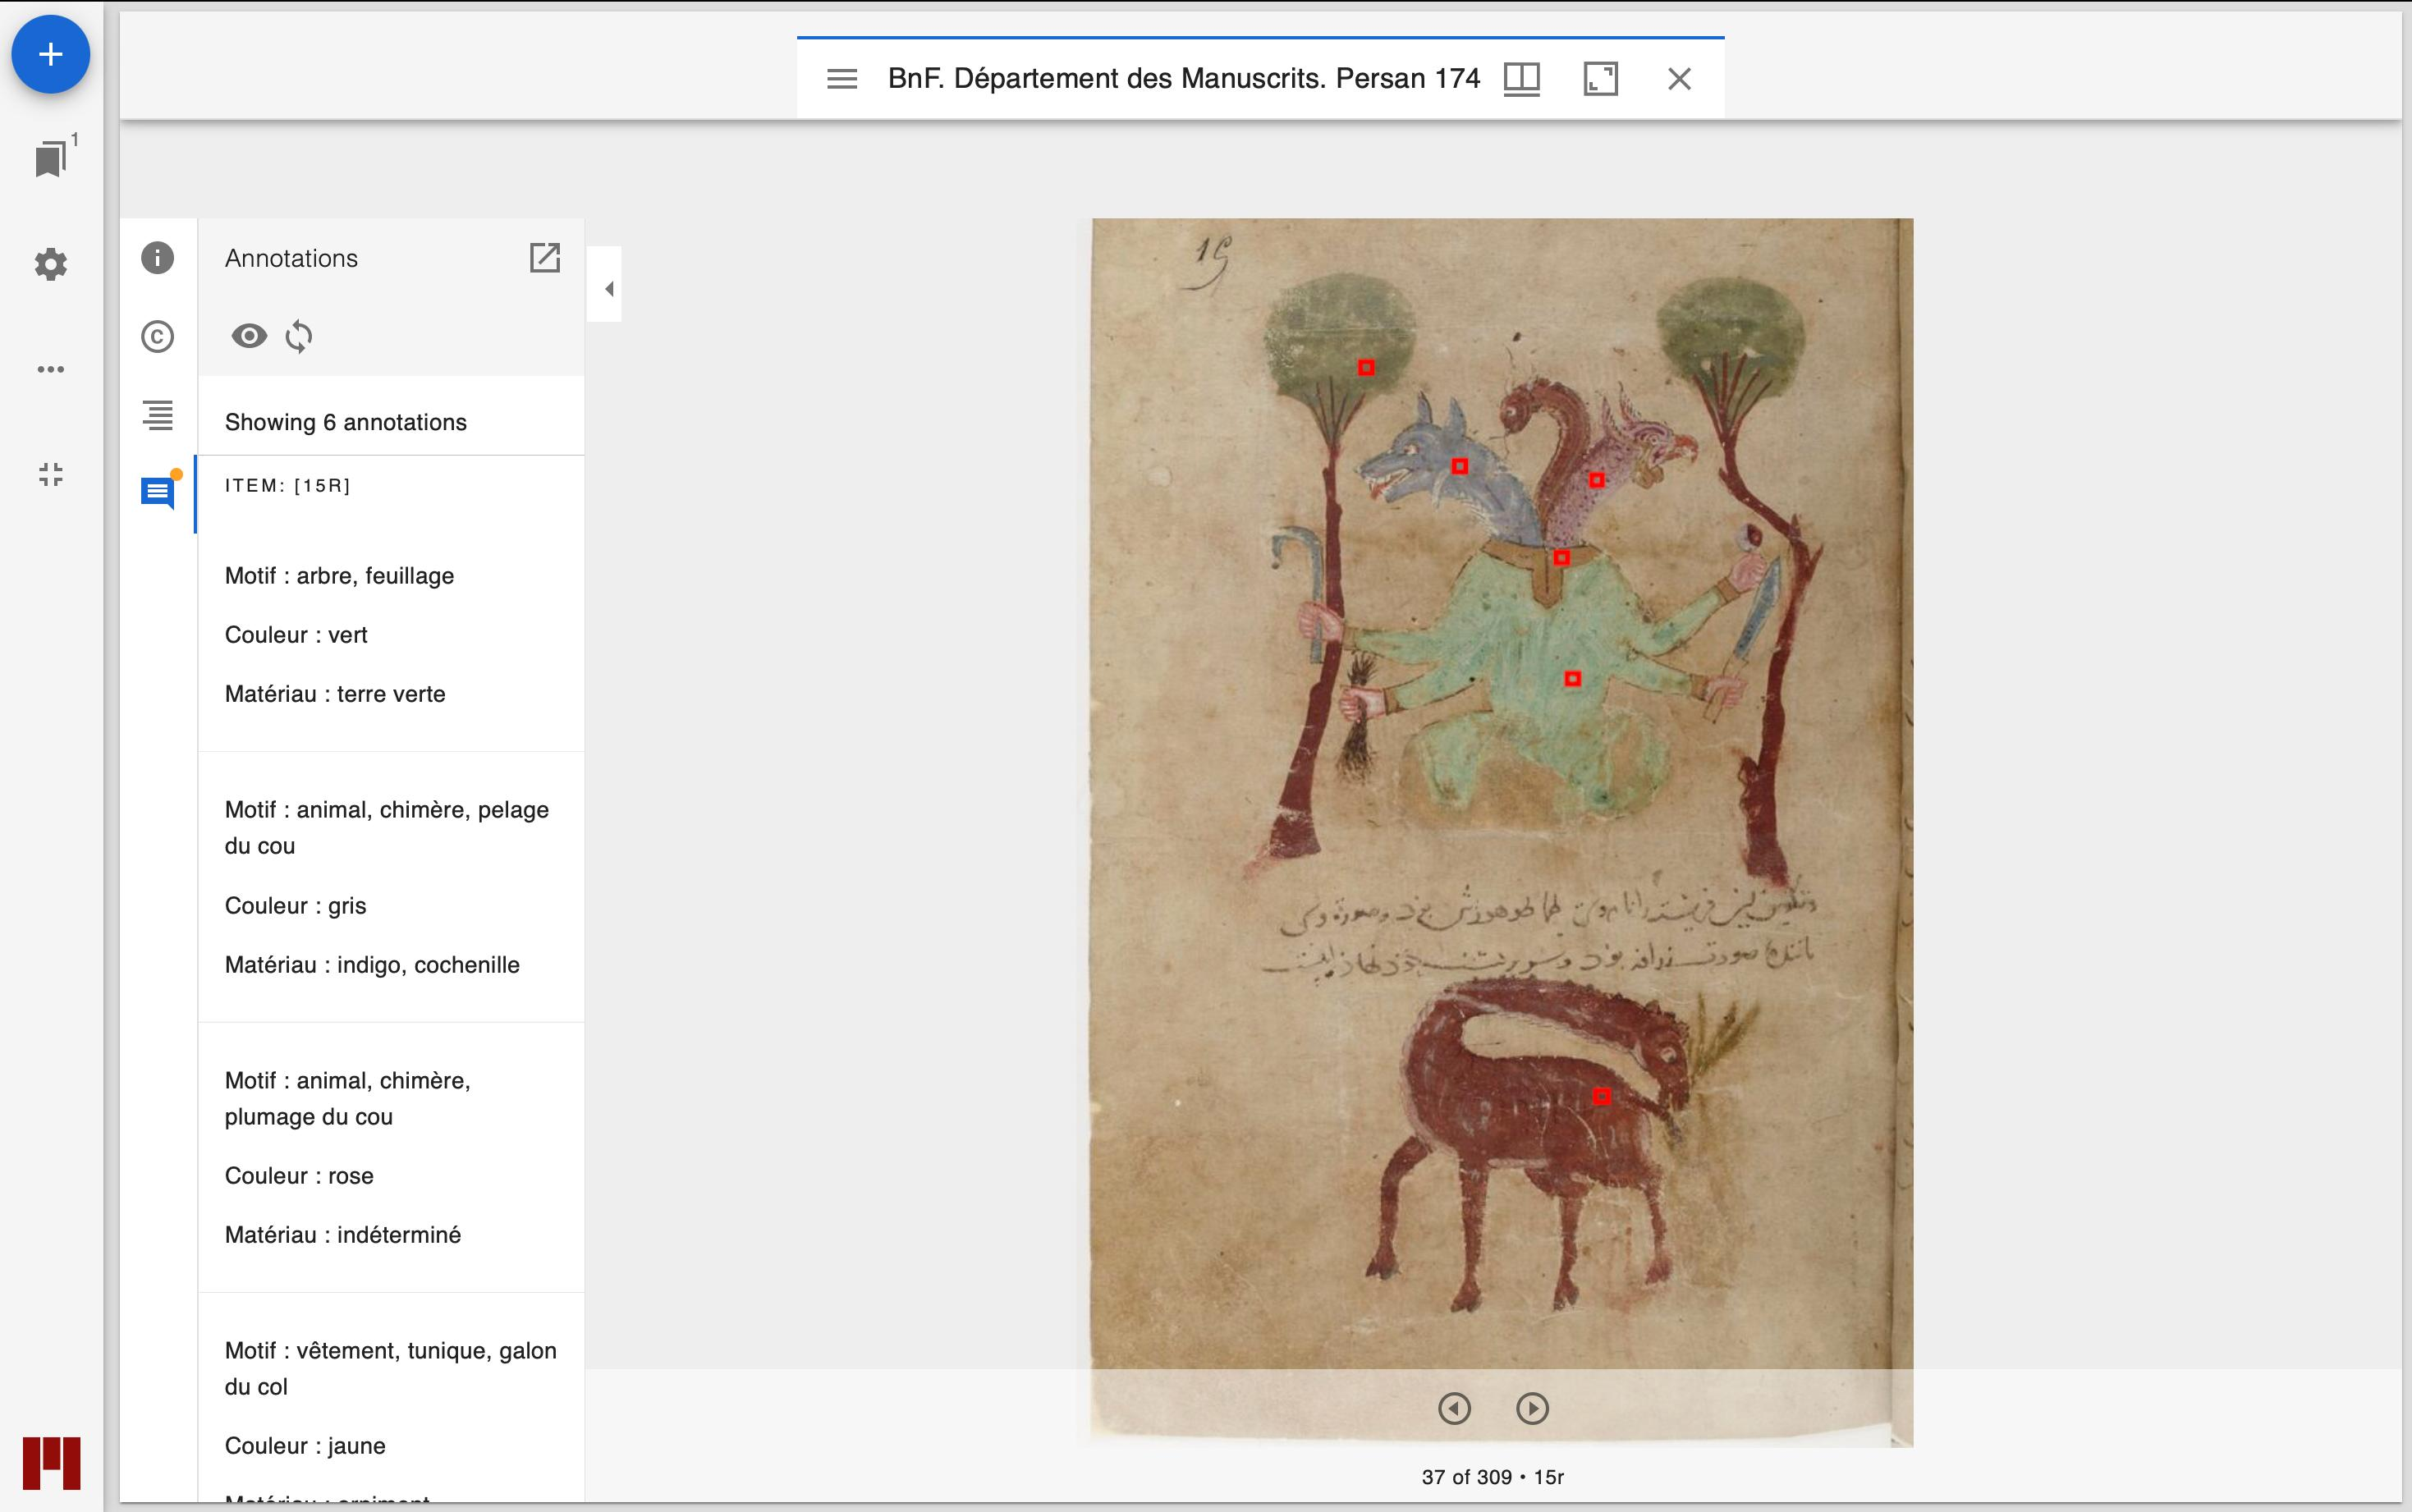
\includegraphics[width=\textwidth]{./textes/annexe/omeka-exemple.jpg}
	\label{fig:info}
\end{figure}